%!TEX root = ../../PhD_thesis__Edouard_Leurent.tex
\graphicspath{{2-Chapters/7-Chapter/}}
	
\chapter{Complements on \Cref{chapter:7}}
	\section{Proofs}
	
	\subsection{Proof of \Cref{prop:regularized_solution}}
	\label{sec:proof-regularized_solution}
	
	\begin{proof}
		We differentiate $J(\theta) = \sum_{n=1}^N \|y_n -\Phi_n\theta\|_{\Sigma_p^{-1}}^2 + \lambda\|\theta\|_{}^2$ as in  \eqref{eq:regression_min} with respect to $\theta$:
		
		\begin{align*}
		\nabla_{\theta} J(\theta) &= \sum_{n=1}^N\nabla_{\theta} (y_n - \Phi_n\theta)^\transp\Sigma_p^{-1}(y_n - \Phi_n\theta) + \nabla_{\theta} \lambda\|\theta\|_{}^2\\
		&= -2\sum_{n=1}^N y_n^\transp\Sigma_p^{-1}\Phi_n + 2\sum_{n=1}^N\theta^\transp(\Phi_n^\transp\Sigma^{-1}\Phi_n) +  2 \lambda \theta^\transp
		\end{align*}
		
		Hence,
		\begin{align*}
		\nabla_{\theta} J(\theta) = 0 \iff \left(\sum_{n=1}^N\Phi_n^\transp\Sigma_p^{-1}\Phi_n + I_d\right)\theta = \sum_{n=1}^N y_n^\transp\Sigma_p^{-1}\Phi_n
		\end{align*}
	\end{proof}
	
	\subsection{Proof of \Cref{thm:confidence_ellipsoid}}
	\label{sec:proof-confidence_ellipsoid}
	
	We start by showing a preliminary proposition:
	\newpage
	
	\begin{proposition}[Matrix version of Theorem 1 of \citealp{Abbasi2011}]
		\label{prop:concentration}
		\begin{leftbar}[propositionbar]
		Let $\{F_n\}_{n=0}$ be a filtration.
		Let $\{\eta_n\}_{n=1}^\infty$ be a $\Real^p$-valued stochastic process such that $\eta_n$ is $F_n$-measurable and $\expectedvalue\left[\eta_n\condbar F_{n-1}\right]$ is $\Sigma_p$-sub-Gaussian.
		
		Let $\{\Phi_n\}_{n=1}^\infty$ be an $\Real^{p\times d}$-valued stochastic process such that $\Phi_n$ is $F_n$-measurable. Assume that $G$ is a $d\times d$ positive definite matrix.
		For any $n\geq 0$, define
		\begin{equation*}
		\overline{G}_n = G + \sum_{s=1}^n \Phi_s^\transp \Sigma_p^{-1} \Phi_s \in \Real^{d\times d} \quad S_n = \sum_{s=1}^n \Phi_s^\transp\Sigma_p^{-1}\eta_s \in \Real^{d}.
		\end{equation*}
		Then, for any $\confidence>0$, with probability at least $1-\confidence$, for all $n\geq0$,
		\begin{align*}
		\| S_n \|_{\overline{G}_n^{-1}} \leq \sqrt{2\log \left(\frac{\det\left(\overline{G}_n\right)^{1/2}}{\confidence\det(G)^{1/2}}\right)}.
		\end{align*}
		\end{leftbar}
	\end{proposition}
	\begin{proof}
		Let 
		\begin{equation*}
		G_t = \sum_{s=1}^t \Phi_s^\transp \Sigma_p^{-1} \Phi_s \in \Real^{d\times d}
		\end{equation*}
		And for any $z\in\Real^d$,
		\begin{equation*}
		M_t^z = \exp{\left(\inp{z}{S_t} - \frac{1}{2}\|z\|_{G_t}\right)}
		\end{equation*}
		\begin{equation*}
		D_t^z = \exp{\left(\inp{\Phi_t z}{\eta_t}_{\Sigma_p^{-1}} - \frac{1}{2}\|\Phi_t z\|_{\Sigma_p^{-1}}\right)}
		\end{equation*}
		Then,
		\begin{align*}
		M_t^z &= \exp{\left(\sum_{s=1}^t z^\transp \Phi_s^\transp \Sigma_p^{-1} \eta_s - \frac{1}{2} (\Phi_s z)^\transp\Sigma_p^{-1}(\Phi_s z) \right)} \\
		&= \prod_{s=1}^{t} D_s^z
		\end{align*}
		and using the sub-Gaussianity of $\eta_t$
		\begin{align*}
		\expectedvalue\left[D_t^z \condbar F_{t-1}\right] = {}& \exp{\left(- \frac{1}{2}\|\Phi_t z\|_{\Sigma_p^{-1}}\right)}\\ &\expectedvalue\left[\exp{\left(\inp{\Phi_t z}{\eta_t}_{\Sigma_p^{-1}}\right)} \condbar F_{t-1}\right]  \\
		\leq {} & \exp{\left(- \frac{1}{2}\|\Phi_t z\|_{\Sigma_p^{-1}}\right)}\\
		&\exp{\left((z^\transp \Phi_t^\transp \Sigma_p^{-1})\Sigma_p(\Sigma_p^{-1} \Phi_t z)\right)}\\
		&= 1
		\end{align*}
		\begin{align*}
		\expectedvalue\left[M_t^z \condbar F_{t-1}\right] = \left(\prod_{s=1}^{t-1} D_s^z\right) \expectedvalue\left[D_t^z \condbar F_{t-1}\right] \leq M_{t-1}^z
		\end{align*}
		Showing that $(M_t^z)_{t=1}^\infty$ is indeed a supermartingale and in fact $\expectedvalue[M_t^z]\leq 1$.
		It then follows by Doob's upcrossing lemma for supermartingale that $M_\infty^z = \lim_{t\to\infty} M_t^z$ is almost surely well-defined, and so is $M_\tau^z$ for any random stopping time $\tau$.
		
		Next, we consider the stopped martingale $M_{\min(\tau,t)}^z$. Since 
		$(M_t^z)_{t=1}^\infty$ is a non-negative supermartingale and $\tau$ is a random stopping time, we deduce by Doob's decomposition that
		\begin{align*}
		\expectedvalue[M_{\min(\tau,t)}^z] &= \expectedvalue[M_0^z] + \expectedvalue[\sum_{s=0}^{t-1} (M_{s+1}^z-M_s^z) \mathbb{I}\{\tau>s\}]\\
		&\leq 1 + \expectedvalue[\sum_{s=0}^{t-1} \expectedvalue[M_{s+1}^z-M_s^z|F_{s}] \mathbb{I}\{\tau>s\}]\\
		&\leq 1
		\end{align*}
		Finally, an application of Fatou's lemma show that 
		$$\expectedvalue[M_\tau^z] = \expectedvalue[\liminf_{t\to\infty} M_{\min(\tau,t)}^z] \leq \liminf_{t\to\infty} \expectedvalue[M_{\min(\tau,t)}^z] \leq 1.$$
		
		This results allows to apply a result from \citep{pena2008self}.
		\begin{lemma}[Theorem 14.7 of \citealp{pena2008self}]
			\begin{leftbar}[lemmabar]
			If $Z$ is a random vector and $B$ is a symmetric positive definite matrix such that
			\[\forall \discount\in\Real^d, \log \expectedvalue \exp \left(\discount^\transp Z -\frac{1}{2} \discount^\transp B \discount \right)\leq 0,\]
			then for any positive definite non-random matrix C, it holds
			\[\expectedvalue\left[ \sqrt{\frac{\det(C)}{\det(B+C)} } \exp\left( \frac{1}{2}\|Z\|^2_{(B+C)^{-1}}\right)\right]\leq 1. \] 
			In particular, by Markov inequality, for all $\confidence\in(0,1)$, 
			\[\probability{\|Z\|_{(B+C)^{-1}} \geq \sqrt{2\log \left(\frac{\det \left((B+C)^{1/2}\right)}{\confidence\det(C)^{1/2}}\right)}}\leq \confidence.\]
			\end{leftbar}
		\end{lemma}
		
		Here, by using $Z = \sum_{s=1}^t\Phi_s\Sigma_p^{-1}\eta_s$, $B=G_t$, $C=G$,
		
		\[
		\probability{\| S_t \|_{(G_t+G)^{-1}} \geq \sqrt{2\log \left(\frac{\det(G_t+G)^{1/2}}{\confidence\det(G)^{1/2}}\right)}} \leq \confidence
		\]
		
	\end{proof}
	
	Having shown this preliminary result, we move on to the proof of \Cref{thm:confidence_ellipsoid}.
	
	\begin{proof}
		For all $x\in\Real^d$, \eqref{eq:vector_rls} gives
		\begin{align*}
		x^\transp\theta_{N,\lambda}  -x^\transp\theta &= x^\transp G_{N, \lambda}^{-1}\sum_{n=1}^N \Phi_n^\transp \Sigma_p^{-1}\eta_n
		- \lambda x^\transp G_{N, \lambda}^{-1}\theta\\
		&= \inp{x}{\sum_{n=1}^N \Phi_n^\transp \Sigma_p^{-1}\eta_n}_{G_{N, \lambda}^{-1}} - \lambda\inp{x}{\theta}_{G_{N, \lambda}^{-1}}
		\end{align*}
		
		Using the Cauchy-Schwartz inequality, we get
		\begin{align*}
		|x^\transp\theta_{N,\lambda}  -x^\transp\theta| \leq \|x\|_{G_{N, \lambda}^{-1}}\left(\left\|\sum_{n=1}^N \Phi_n^\transp \Sigma_p^{-1}\eta_n\right\|_{G_{N, \lambda}^{-1}} + \lambda\|\theta\|_{G_{N, \lambda}^{-1}}\right)
		\end{align*}
		
		In particular, for $x = G_{N,\lambda}(\theta_{N,\lambda} - \theta)$, we get after simplifying with $\| \theta_{N,\lambda}  - \theta\|_{G_{N,\lambda}}$,
		\begin{align*}
		\| \theta_{N,\lambda}  - \theta\|_{G_{N,\lambda}} &\leq \left\|\sum_{n=1}^N \Phi_n^\transp \Sigma_p^{-1}\eta_n\right\|_{G_{N, \lambda}^{-1}} + \lambda\|\theta\|_{G_{N, \lambda}^{-1}}
		\end{align*}
		
		By applying \Cref{prop:concentration} with $G=\lambda I_d$, we obtain that with probability at least $1-\confidence$,
		\begin{align*}
		\| \theta_{N,\lambda}  - \theta\|_{G_{N,\lambda}} &\leq \sqrt{2\log \left(\frac{\det(G_{N,\lambda})^{1/2}}{\confidence\det(\lambda I_d)^{1/2}}\right)}
		+ \lambda\|\theta\|_{G_{N, \lambda}^{-1}}
		\end{align*}
		And since $\|\theta\|_{G_{N, \lambda}^{-1}}^2 \leq 1/\lambda_{\min}(G_{N,\lambda})\|\theta\|_2^2 \leq 1/\lambda \|\theta\|_2^2$ and $\|\theta\|_2^2 \leq d\|\theta\|_\infty^2\leq d S^2$,
		\begin{align*}
		\| \theta_{N,\lambda}  - \theta\|_{G_{N,\lambda}} &\leq \sqrt{2\log \left(\frac{\det(G_{N,\lambda})^{1/2}}{\confidence\det(\lambda I_d)^{1/2}}\right)}
		+ (\lambda d)^{1/2}S
		\end{align*}
	\end{proof}
	
	
	\subsection{Proof of \Cref{prop:lower-bound}}
	\label{sec:proof-lower-bound}
	\begin{proof}
		The predictor designed in \Cref{sec:prediction} verifies the inclusion property \eqref{eq:inclusion-property}. Thus, for sequence of controls $\bu$, any dynamics $\structureddynamics\in C_{[N],\confidence}$, and perturbations $\underline{\omega} \leq \omega \leq \overline{\omega}$, the corresponding state at time $t_n$ is bounded by $\underline{x}_n \leq x_n \leq \overline{x}_n$, which implies that $R(x_n) \geq \min_{x\in[\underline{x}_n(\bu), \overline{x}_n(\bu)]}  R(x) = \pessimisticreward_n(\bu)$.
		
		Thus, by taking the min over $C_{[N],\confidence}$ and $[\underline{\omega}, \overline{\omega}]$, we also have for any sequence of controls $\bu$,
		\begin{align*}
		V^r(\bu) &= \min_{\substack{\structureddynamics\in C_{[N],\confidence}\\ \underline{\omega} \leq \omega \leq \overline{\omega}}} \sum_{n=N+1}^\infty \discount^n R(x_n)\\
		&\geq \sum_{n=N+1}^\infty \discount^n \pessimisticreward_n(\bu)\\
		&= \hat{V}^r(\bu)
		\end{align*}
	\end{proof}
	
	\subsection{Proof of \Cref{thm:minimax-regret-bound}}
	\label{sec:proof-minimax-regret-bound}
	We first bound the model estimation error.
	\begin{lemma}
	\label{lem:dynamics-est-bound}
	\begin{leftbar}[lemmabar]
		\[\|A(\theta) - A(\theta_{N,\lambda})\|_F = \cO\left(\sqrt{ {\frac{\beta_N(\delta)^2}{\lambda_{\min}(G_{N,\lambda})}}}\right) \]
	\end{leftbar}
	\end{lemma}
	\begin{proof}
	We have 
	\begin{align*}
	\|\theta - \theta_{N,\lambda}\|_{G_{N,\lambda}}^2 \geq \lambda_{\min}(G_{N,\lambda})\|\theta - \theta_{N,\lambda}\|_{2}^2
	\end{align*}
	And \eqref{eq:confidence-ellipsoid} gives
	\[\|\theta - \theta_{N,\lambda}\|_{G_{N,\lambda}}^2 = \cO(\beta_N(\delta)^2) \]
	
	Moreover, $A(\theta)$ belongs to a linear image of this $L^2$-ball. By writing a the $j^{th}$ column of a matrix $M$ as $M_j$, and its coefficient $i,j$ as $M_{i,j}$,
	\begin{align*}
	((A(\theta)-A(\theta_{N,\lambda}))^\transp (A(\theta) - A(\theta_{N,\lambda})))_{i,j}
	&= (\theta-\theta_{N,\lambda})^\transp\phi_{i}^{\transp}\phi_j(\theta-\theta_{N,\lambda}) \\
	&\leq \lambda_{\max}(\phi_{i}^{\transp}\phi_j) \|\theta - \theta_{N,\lambda}\|_{2}^2
	\end{align*}
	
	Thus, $\|A(\theta) - A(\theta_{N,\lambda})\|_F^2 = \Tr{\left[(A(\theta)-A(\theta_{N,\lambda}))^\transp (A(\theta) - A(\theta_{N,\lambda}))\right]} = \cO\left( {\frac{\beta_N(\delta)^2}{\lambda_{\min}(G_{N,\lambda})}}\right)$
	\end{proof}
	
	Then, we propagate this estimation error through the state prediction.
	
	\begin{lemma}
		\begin{leftbar}[lemmabar]
		If there exist $P>0,Q_0\in\Real^{p\times p}$, $\rho>0$ such that
		\begin{align*}
		\begin{bmatrix}
		A_N^\transp P + P A_N + Q_0 & P|D|  \\
		|D|^\transp P & -\rho I_r \\
		\end{bmatrix}< 0,
		\end{align*}
		then for all $t> t_N$,
		\[\|\ox(t) - \ux(t)\| \leq \left(C_0 + \cO\left({\frac{\beta_N(\delta)}{\sqrt{\lambda_{\min}(G_{N,\lambda})}}} \right)\right)C_\omega(t), \]
		where $$C_0 = \sqrt{\frac{2\rho\lambda_{\max}(P)}{\lambda_{\min}(P)\lambda_{\min}(Q_0)}},$$ and $$C_\omega(t) = \sup_{\tau\in[0,t]} \|\overline{\omega}(\tau) - \underline{\omega}(\tau)\|_2.$$
		\end{leftbar}
	\end{lemma}
	\begin{proof}
		Let $e = \ox - \ux$. \eqref{eq:interval-predictor} gives the dynamics
		\begin{align*}
		\dot{e} = A_Ne + |\Delta A|(\ox^+ + \ux^-) + |D|(\overline{\omega} - \underline{\omega})
		\end{align*}
		where recall that $|M| = M^+ + M^-$ for any matrix $M\in\Real^{p\times p}$.
		
		We define the Lyapunov function $V = e^\transp P e$, which is non-negative definite provided that
		$
		P>0,
		$ and compute its derivative
		\begin{align*}
		\dot{V} ={}& X^\transp
		\begin{bmatrix}
		A_N^\transp P + P A_N + Q & P|D| & P|\Delta A| \\
		|D|^\transp P & -\rho I_r & 0\\
		|\Delta A|^\transp P & 0 & -\alpha I_p
		\end{bmatrix}
		X\\
		& - e^\transp Q e + \alpha |\ux^+ + \ox^-|^2 + \rho |\overline{\omega} - \underline{\omega}|^2
		\end{align*}
		with $X=\begin{bmatrix}
		e & \overline{\omega} - \underline{\omega} &  \ux^+ + \ox^-
		\end{bmatrix}^\transp$, for any $Q\in\Real^{p\times p}$, $\rho,\alpha\in\Real$ . 
		
		Moreover, it holds that $-\ux^+ -\ox^- \leq e \leq \ox^+ + \ux^-$, which implies $|\ux^+ + \ox^-| \leq 2 |e|$. Hence,
		\begin{align*}
		\dot{V} \leq {}& X^\transp
		\underbrace{
			\left[
			\begin{array}{cc|c}
			A_N^\transp P + P A_N + Q + 4\alpha I_p & P|D| & P|\Delta A| \\
			|D|^\transp P & -\rho I_r & 0\\
			\hline
			|\Delta A|^\transp P & 0 & -\alpha I_p
			\end{array}
			\right]}_{\Upsilon}
		X\\
		& - e^\transp Q e + \rho \|\overline{\omega} - \underline{\omega}\|_2^2
		\end{align*}
		
		Thus, if we had $\Upsilon \leq 0$, $Q>0$, $\rho > 0$, then we would have
		\[
		\dot{V} \leq -\mu V + \rho \|\overline{\omega} - \underline{\omega}\|_2^2
		\]
		with $\mu = \frac{\lambda_{\min}(Q)}{\lambda_{\max}(P)}$. Since $V(t_N) = 0$, this further implies that for all $t>t_N$, 
		\begin{equation}
		\label{eq:lyap-bound}
		V(t) \leq \frac{\rho}{\mu} C_\omega^2(t)
		\end{equation}
		
		We now examine the condition $\Upsilon \leq 0$.
		We resort to its Schur complement: given $\alpha > 0$, $\Upsilon \leq 0$ if and only if $R \geq S$, where $S= \alpha^{-1}\begin{bmatrix}|\Delta A|^\transp P & 0\end{bmatrix}^\transp \begin{bmatrix}|\Delta A|^\transp P & 0\end{bmatrix}$ and $R$ is the top-left block of $-\Upsilon$:
		\[R = \begin{bmatrix}
		-A_N^\transp P - P A_N - Q - 4\alpha I_p & -P|D|\\
		-|D|^\transp P & \rho I_r\\
		\end{bmatrix}\]
		
		Choose $Q = \frac{1}{2}Q_0-4\alpha I_p$.
		Assume that $P$ is fixed and satisfies the conditions of the lemma. We have 
		\begin{align*}
		\lambda_{\max}(S) &\leq \alpha^{-1}\lambda_{\max}(P)^2\lambda_{\max}(|\Delta A|^\top |\Delta A|)\\
		&\leq\alpha^{-1}\lambda_{\max}(P)^2\|\Delta A\|_F^2
		\end{align*}
		
		
		Thus, by taking $\alpha = \frac{2\lambda_{\max}(P)^2\|\Delta A\|_F^2}{\lambda_{\min}(Q_0)} = \cO({\frac{\beta_N(\delta)^2}{\lambda_{\min}(G_{N,\lambda})}})$, we can obtain that $S \leq \begin{bmatrix}
		\frac{1}{2}Q_0 & 0\\0 & 0
		\end{bmatrix}$. Thus,
		\[R-S \geq \begin{bmatrix}
		-A_N^\transp P - P A_N - Q_0 & -P|D|\\
		-|D|^\transp P & \rho I_r\\
		\end{bmatrix} > 0 \]
		as it is assumed in the conditions of the lemma. Hence, under such a choice of $\alpha$ and $Q$, we recover $\Upsilon\leq 0$. \eqref{eq:lyap-bound} follows with $\mu = \frac{\lambda_{\min}(Q)}{\lambda_{\max}(P)} = \frac{\frac{1}{2}\lambda_{\min}(Q_0) - 4\alpha}{\lambda_{\max}(P)}$.
		Finally, we obtain
		\begin{align*}
		\|e(t)\|_2^2 &\leq \lambda_{\min}(P)^{-1} V(t)\\
		& \leq \frac{2\rho\lambda_{\max}(P)/\lambda_{\min}(P)}{\lambda_{\min}(Q_0) - 8\alpha} C_\omega^2(t)\\
		\end{align*}
		Developing at the first order in $\alpha$ gives
		\begin{align*}
		\|e(t)\|_2 &\leq C_0\left(1 + \frac{4\alpha}{\lambda_{\min}(Q_0)} + \cO(\alpha^2)\right)C_\omega(t)\\
		&\leq \left(C_0 + \cO\left({\frac{\beta_N(\delta)^2}{\lambda_{\min}(G_{N,\lambda})}}\right)\right)C_\omega(t)
		\end{align*}
	\end{proof}
	
	
	Finally, we propagate the state prediction error bound to the pessimistic rewards and surrogate objective to get our final result.
	\begin{proof}
		For any sequence of controls $\bu$, dynamical parameters $\theta\in C_{N,\delta}$ and disturbances $\underline{\omega} \leq \omega \leq \overline{\omega}$, we clearly have 
		\[V(\bu)^r \leq V(\bu) = \expectedvalue_{\omega}\sum_n \gamma^n R(x_n)\]
		
		Moreover, by the inclusion property \eqref{eq:inclusion-property}, we have that $\underline{x}_n \leq x_n \leq \overline{x}_n$, which implies that $R(x_n) \leq \max_{x\in[\underline{x}_n(\bu), \overline{x}_n(\bu)]}  R(x)$. Assuming $R$ is $L$-lipschitz,
		\begin{align*}
		V(\bu) - \hat{V}^r(\bu) &\leq \sum_{n=N+1}^\infty \gamma^n \underset{{x\in[\underline{x}_n(\bu), \overline{x}_n(\bu)]}}{(\max - \min)} R(x)\\
		&\leq \sum_{n=N+1}^\infty \gamma^n L \left\|\underline{x}_n(\bu) - \overline{x}_n(\bu)\right\|_2\\
		&\leq L\left(C_0 + \cO\left({\frac{\beta_N(\delta)^2}{\lambda_{\min}(G_{N,\lambda})}}\right)\right) \sum_{n>N} \gamma^n C_{\omega}(t_n)\\
		&= \Delta_\omega + \cO\left({\frac{\beta_N(\delta)^2}{\lambda_{\min}(G_{N,\lambda})}}\right)
		\end{align*}
		with $\Delta_\omega = L C_0\sum_{n>N} \gamma^n C_{\omega}(t_n)$, which is finite by \Cref{assumpt:bounded-noise}.
		
		Finally, we use the result of \Cref{theorem:opd-regret} to account for planning with a finite budget, and relate $\hat{V}^r(a^\star)$ to $\hat{V}^r(a_K)$.
	\end{proof}
	
	\subsection{Proof of \Cref{cor:pe}}
	\label{sec:proof-pe}
	
	\begin{proof}
		By \eqref{eq:vector_rls} and \eqref{eq:pe}, we have $$\lambda_{\min}(G_{N,\lambda}) \geq (N-n_0)\underline{\phi}^2 + \sum_{n<n_0}\Phi_{n}^\transp\Sigma_{p}^{-1}\Phi_{n}$$
		
		and by \eqref{eq:confidence-ellipsoid},
		\begin{align*}
		\beta_N(\delta) &= \sqrt{2\log \left(\frac{\det(G_{N,\lambda})^{1/2}}{\delta\det(\lambda I_d)^{1/2}}\right)}
		+ (\lambda d)^{1/2}S\\
		&\leq \sqrt{\log \left(N^{d/2}\overline{\phi}^d / (\delta\lambda^{d/2})\right)} + \cO(1)
		\end{align*}
		Thus,
		\[
		\frac{\beta_N(\delta)^2}{\lambda_{\min}(G_{N,\lambda})} = \cO\left(\frac{\log (N^{d/2}/\delta)}{N} \right)
		\]
		
		\paragraph{Stability condition 2.}
		
		By \Cref{lem:dynamics-est-bound} and the above, the sequence $(A_N)_{N}$ converges to $A(\theta)$ in Frobenius norm. Thus, 
		$$M_n \eqdef \begin{bmatrix}
		A_N^\transp P + P A_N + Q_0 & P|D|  \\
		|D|^\transp P & -\rho I_r \\
		\end{bmatrix}\text{ also converges to } M\eqdef\begin{bmatrix}
		A(\theta)^\transp P + P A(\theta) + Q_0 & P|D|  \\
		|D|^\transp P & -\rho I_r \\
		\end{bmatrix},$$ which is assumed to be negative definite.
		
		Moreover, the two functions that map a matrix to its characteristic polynomial and a polynomial to its roots, are both continuous. Thus, by continuity, the largest eigenvalue of $M_n$ converges to that of $M$, which is strictly negative. Hence, there exists some $N_0\in\Natural$ such that for all $N>N_0$, $M_N$ is negative definite, as required in the condition 2. of \Cref{thm:minimax-regret-bound}.
	\end{proof}
	
	\subsection{Proof of \Cref{theorem:drop-regret}}
	\label{sec:proof-drop-regret}
		
	We start by showing the following lemma:
	
	\begin{lemma}[Robust values ordering]
		\label{lemma:uvb}
		\begin{leftbar}[lemmabar]
		In addition to the robust U-value defined in \eqref{eq:robust-b-values}, that we extend to inner nodes	
		\begin{equation}
		\label{eq:br}
		U_a^r(k)  \eqdef
		\begin{cases}
		\min_{m\in[M]} \sum_{n=0}^{h-1} \discount^n R_n^m  + \frac{\discount^h}{1-\discount}&\text{if } a \text{ is a leaf;}\\
		\max_{b\in\mathcal{A}} U_{ab}^r(k) & \text{else.}
		\end{cases},
		\end{equation}
		
		we also define the robust value of a sequence of actions $a$
		\begin{equation}
		\label{eq:max_vr}
		V_a^r \eqdef \max_{\bu \in a\mathcal{A^\infty}} \min_{m\in[M]} \sum_{n=h(a)+1}^\infty \discount^n R^m_n
		\end{equation}
		and the robust U-values of a sequence of action $a$
		\begin{equation}
		\label{eq:ur}
		L_a^r(K)  \eqdef
		\begin{cases}
		\min_{m\in[M]} \sum_{n=0}^{h-1} \discount^n R_n^m &\text{if } a \text{ is a leaf;}\\
		\max_{b\in\mathcal{A}} L_{ab}^r(n) & \text{else.}
		\end{cases}
		\end{equation}
		
		Then, the robust values, L-values and U-values exhibit similar properties as the optimal values, L-values and U-values, that is: for all $0 < k < K$ and $a\in\Tau$,
		\begin{equation}
		L^r_a(k) \leq L^r_a(K) \leq V^r_a \leq U^r_a(K) \leq U^r_a(k)
		\end{equation}
		\end{leftbar}
	\end{lemma}
	\begin{proof}
		By definition, when starting with sequence $a$, the value $L_a^m(k)$ represents the minimum admissible reward, while $U_a^m(k)$ corresponds to the best admissible reward achievable with respect to the the possible continuations of $a$. Thus, for all $a\in\mathcal{A}^{\star}$, $L_a^m(k)$ and $L_a^r(k)$ are non-decreasing functions of $k$ and $U_a^m(k)$ and $U_a^r(k)$ are a non-increasing functions of $k$, while $V_a^m$ and $V_a^r$ do not depend on $k$.
		
		Moreover, since the reward function $R$ is assumed be bounded in $[0, 1]$, the sum of discounted rewards from a node of depth $d$ is at most $\discount^d + \discount^{d+1}+\dots = \frac{\discount^d}{1-\discount}$. As a consequence, for all $k \geq 0$ , $a\in\mathcal{L}_k$ of depth $d$, and any sequence of rewards $(R_n)_{n\in\mathbb{N}}$ obtained from following a path in $a\mathcal{A}^\infty$ with any dynamics $m \in [M]$:
		\begin{equation*}
		U^m_a(k) = \sum_{n=0}^{d-1} \discount^n R_n^m \leq \sum_{n=0}^\infty \discount^n R_n^m \leq \sum_{n=0}^{d-1} \discount^n R_n^m + \frac{\discount^d}{1-\discount} = B^m_a(k) 
		\end{equation*}
		Hence,
		\begin{equation}
		\label{eq:min_m_values}
		\min_{m \in [M]} U^m_a(k) \leq \min_{m \in [M]} \sum_{n=0}^\infty \discount^n R_n \leq \min_{m \in [M]} B^m_a(k)
		\end{equation}
		And as the left-hand and right-hand sides of \eqref{eq:min_m_values} are independent of the particular path that was followed in $a\mathcal{A}^\infty$, it also holds for the robust path
		\begin{equation*}
		\min_{m \in [M]} U^m_i(k) \leq \max_{a'\in a\mathcal{A}^\infty} \min_{m \in [M]} \sum_{t=0}^\infty \discount^n R_n^m \leq \min_{m \in [M]} B^m_i(k)
		\end{equation*}
		that is,
		\begin{equation}
		\label{eq:urvrbr}
		L^r_a(k) \leq V^r_a  \leq U^r_a(k)
		\end{equation}
		
		Finally, \eqref{eq:urvrbr} is extended to the rest of $\mathcal{T}_k$ by recursive application of \eqref{eq:max_vr}, \eqref{eq:ur} and \eqref{eq:br}.
	\end{proof}
	
	We now turn to the proof of the theorem.
	
	\begin{proof}
		\citet{Hren2008} first show in Theorem 2 that the simple regret $r_K$ of their optimistic planner is bounded by $\frac{\discount^{d_K}}{1 - \discount}$ where $d_K$ is the depth of $\mathcal{T}_K$. This properties relies on the fact that the returned action belongs to the deepest explored branch, which we can show likewise by contradiction using \Cref{lemma:uvb}. This yields directly that the returned action $a = i_0$ where $i$ is some node of maximal depth $d_K$ expanded at round $k\leq K$, which by selection rule verifies $U_a^r(k) = U_i^r(k) = \max_{x\in\mathcal{A}} U_x^r(k)$ and
		\begin{align*}
		\label{eq:Rndn}
		V^r - V_a^r &= V_{a^{\star}}^r - V_a^r  \\
		&\leq U_{a^{\star}}^r(k) - V_a^r \\
		&\leq U_{a}^r(k) - L_a^r(k) \\
		&= U_{i}^r(k) - L_i^r(k) \\
		&= \frac{\discount^{d_K}}{1-\discount}.
		\end{align*}
		
		Secondly, they bound the depth $d_K$ of $\mathcal{T}_K$ with respect to $K$. To that end, they show that the expanded nodes always belong to the sub-tree $\mathcal{T}_\infty$ of all the nodes of depth $d$ that are $\frac{\discount^d}{1-\discount}$-optimal. Indeed, if a node $i$ of depth $d$ is expanded at round $k$, then $U_i^r(k) \geq U_j^r(k)$ for all $j\in \mathcal{L}_k$ by selection rule, thus the max-backups of \eqref{eq:robust-b-values} up to the root yield $U^r_i(k) = U_\emptyset^r(k)$. Moreover, by \Cref{lemma:uvb} we have that $U_\emptyset^r(k) \geq V_\emptyset^r = V^r$ and so $V_i^r \geq L_i^r(k) = U_i^r(k) - \frac{\discount^d}{1-\discount} \geq V^r - \frac{\discount^d}{1-\discount}$, thus $i \in \mathcal{T}_\infty$.
		
		Then from the definition of $\kappa$ applied to nodes in $\mathcal{T}_\infty$, there exists $d_0$ and $c$ such that the number $n_d$ of nodes of depth $d \geq d_0$ in $\mathcal{T}_\infty$ is bounded by $c\kappa^d$. As a consequence, 
		\begin{eqnarray*}
			K &= \sum_{d=0}^{d_K} n_d = n_0 + \sum_{d=d_0+1}^{d_K} n_d \leq n_0 + c\sum_{d={d_0+1}}^{d_K} \kappa^d.
		\end{eqnarray*}
		
		\begin{itemize}
			\item If $\kappa > 1$, then $K \leq n_0 + c\kappa^{d_0+1}\frac{\kappa^{d_K-d_0}-1}{\kappa-1}$ and thus $d_K \geq d_0 + \log_\kappa \frac{(K-n_0)(\kappa - 1)}{c\kappa^{d_0+1}}$.
			
			We conclude that $r_K \leq \frac{\discount^{d_K}}{1-\discount} = \frac{1}{1-\discount} \left( \frac{(K-n_0)(\kappa - 1)}{c\kappa^{d_0+1}} \right)^\frac{\log \discount}{\log \kappa} = \cO\left(K^{-\frac{\log 1/\discount}{\log \kappa}}\right)$.
			
			\item If $\kappa = 1$, then $K \leq n_0 + c(d_K-d_0)$, hence we have $r_K = O\left(\discount^{Kc}\right)$.
		\end{itemize}
	\end{proof}
	
%	\subsection{Description of attached files}
%	\label{sec:attachments}
%	
%	\paragraph{Videos}
% The \texttt{video} folder contains videos comparing trajectories of the oracle planner and \Cref{alg:full}. The oracle planner has access to the true dynamics and follows aggressive trajectories that nearly saturate the collision constraints. In contrast, the \Cref{alg:full} produces more conservative trajectories. In the obstacle experiment, we show the confidence ellipsoid over $\theta = (\theta_x,\theta_y)$ in the right panel. In the driving experiment, we show the multi-model rejection and robust selection procedure through the display of several trajectory hulls for all possible destinations of the observed vehicles.
%	
% \paragraph{Source code}
%	The attached \texttt{code} directory contains an implementation of \Cref{alg:full}. We relate the algorithmic steps of this chapter to their location in the source code.
%	\begin{enumerate}
%		\item The confidence ellipsoid \eqref{eq:confidence-ellipsoid} is implemented in the \texttt{ellipsoid()} method in \url{code/rl_agents/agents/tree_search/robust_epc.py}
%		\item The corresponding polytope \eqref{eq:polytope} is implemented in the \texttt{polytope()} method of \url{code/rl_agents/agents/tree_search/robust_epc.py}
%		\item The simple predictor of \eqref{eq:predictor-naive} is implemented in the \texttt{step\_simple\_predictor()} method of \url{code/rl_agents/agents/common/interval.py}
%		\item The enhanced predictor of \eqref{eq:interval-predictor} is implemented in the \texttt{step\_interval\_predictor()} method of \url{code/rl_agents/agents/common/interval.py}
%		\item The pessimistic reward of \eqref{eq:pessimistic-rewards} is implemented in the \texttt{pessimistic\_reward()} method of \url{code/obstacle_env/envs/obstacle.py} and the \texttt{check\_collision()} method of \url{code/highway_env/vehicle/uncertainty/prediction.py}
%		\item The robust upper-bound of \eqref{eq:robust-b-values} is implemented in the \texttt{RobustNode} class of \url{code/rl_agents/agents/tree_search/robust.py}
%	\end{enumerate}
%%	The experiments can be reproduced by running
%%	\lstset{language=bash}
%%	\begin{lstlisting}
%%	cd scripts
%%	python experiments.py configs/<env>/env.json configs/<env>/agents/<agent>.json
%%	\end{lstlisting}
%	
	
	\section{A tighter enclosing polytope}
	\label{sec:tight-polytope}
	
%	\begin{figure}[ht]
%		\centering
%		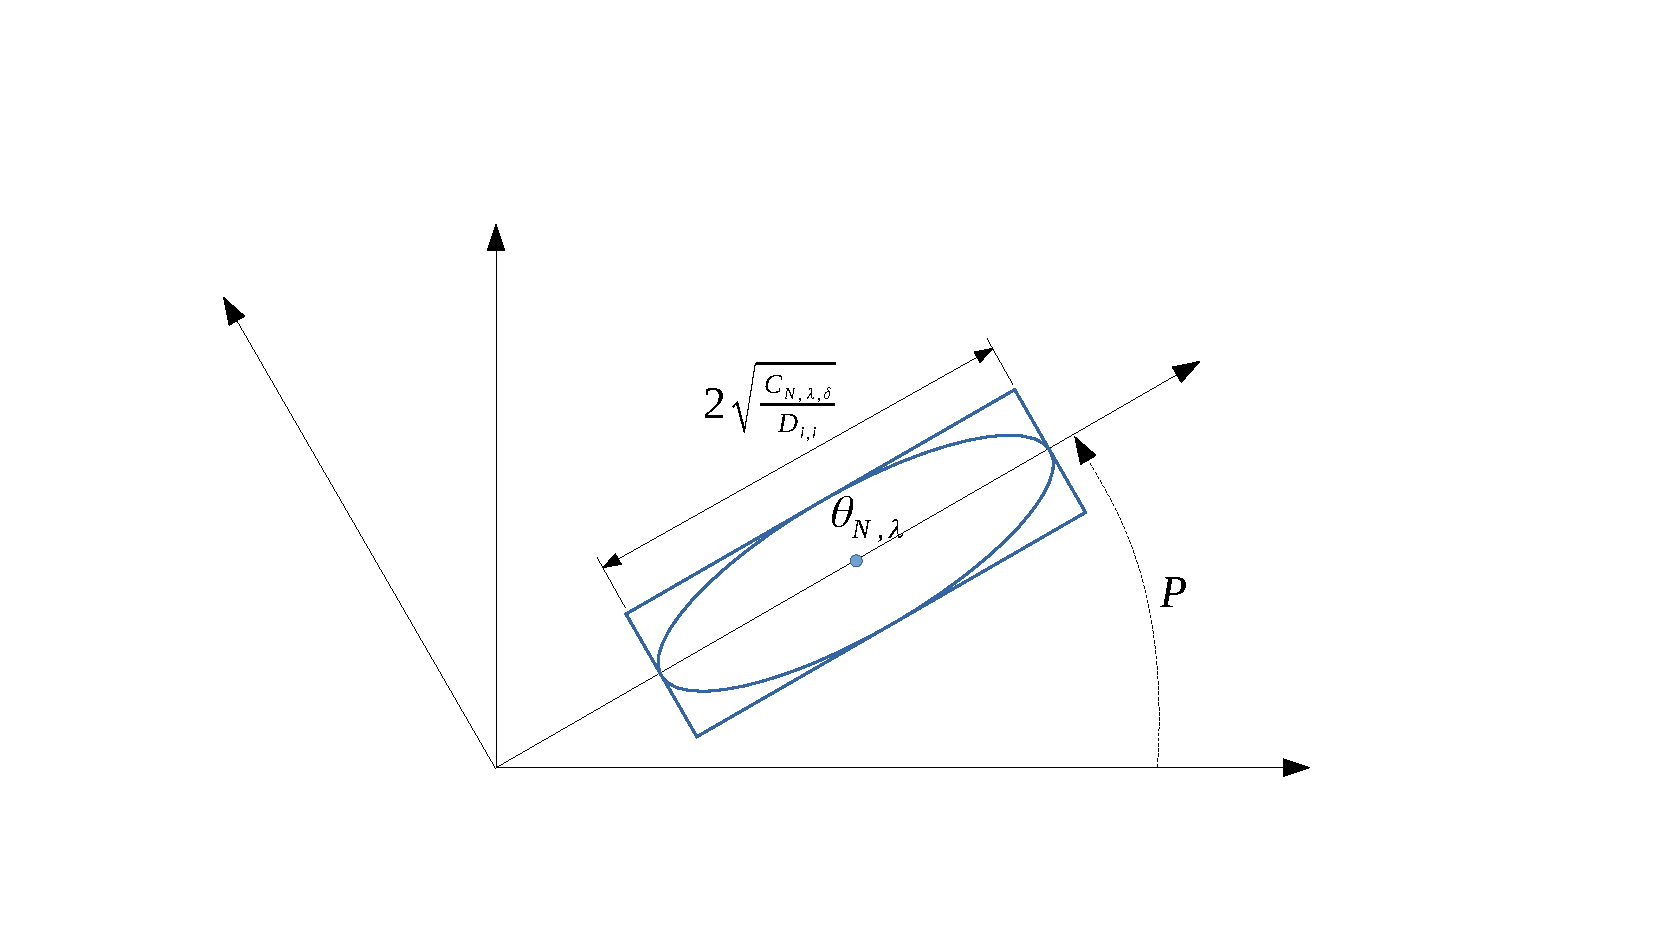
\includegraphics[trim={3.8cm, 2cm, 5cm, 3.8cm}, clip, width=0.7\linewidth]{img/ellipsoid_to_polytope}
%		\caption{From the confidence ellipsoid $\cC_\confidence$ to its enclosing polytope $\cP_\confidence$}
%		\label{fig:ellipsoid_to_polytope}
%	\end{figure}
	
	\begin{lemma}[Confidence polytope]
		\label{lem:tight_polytope}
		\begin{leftbar}[lemmabar]
		We can enclose the confidence ellipsoid obtained in $\eqref{eq:confidence-ellipsoid}$ within a polytope
		\begin{equation}
		\cP = \left\{ A_{0}+\sum_{i=1}^{2^d}\lambda_{i}\Delta A_{i}: \lambda\in[0, 1]^{2^d},  \sum_{i=1}^{2^d}\lambda_{i}=1\right\}.
		\end{equation}
		with 
		\begin{align*}
		&h_k \text{ is the }k^\text{th}\text{ element of }\{-1,1\}^d\text{ for } k\in[2^d],\\
		&G_{N,\lambda} = PDP^{-1}, \quad \Delta\theta_k = \beta_{N}(\confidence)^{1/2} P^{-1}D^{-1/2} h_k, \\
		&A_0 = A + \theta_{N,\lambda}^\transp\phi, \quad \Delta A_k = \Delta\theta_k^\transp\phi.
		\end{align*}
		This conversion is illustrated in \Cref{fig:ellipsoid_to_polytope}.
		\end{leftbar}
	\end{lemma}

	\begin{proof}
		The ellipsoid in \eqref{eq:confidence-ellipsoid} is described by
		\begin{align*}
		\theta\in\confidenceset &\implies
		(\theta-\theta_{N,\lambda})^\transp G_{N,\lambda}(\theta-\theta_{N,\lambda}) \leq \beta_{N}(\confidence)\\
		&\implies (\theta'-\theta'_{N,\lambda})^\transp D (\theta'-\theta'_{N,\lambda}) \leq \beta_{N}(\confidence)\\
		&\implies \sum_{i=1}^d D_{i,i}(\theta'_i-\theta'_{N,\lambda,i})^2\leq \beta_{N}(\confidence)\\
		&\implies\forall i, |\theta'_i-\theta'_{N,\lambda,i}|\leq \beta_{N}(\confidence)^{1/2}D_{i,i}^{-1/2}
		\end{align*}
		This describes a $\Real^d$ box containing $\theta' = P\theta$, whose $k^\text{th}$ vertex is represented by $$\theta_{N,\lambda}' + \beta_{N}(\confidence)^{1/2}D^{-1/2} h_k.$$ We obtain the corresponding box on $\theta$ by transforming each vertex of the box with $P^{-1}$.
	\end{proof}

	
%		
%	\subsection{Experimental setting}
%	\label{sec:experimental-setting}
%	
%	In both experiments, we used $\discount=0.9$,  $\confidence=0.9$ and a planning budget $K=100$. The perturbations were sampled uniformly in $[-0.1, 0.1]^r$ while the measurements are Gaussian with covariance $\Sigma_r = 0.1 I_s$. 
%	
%	\subsection{Autonomous Driving}
%	
%	In the following, we describe the structure of the dynamical system $f$ representing the couplings and interactions between several vehicles.
%	
%	\paragraph{Kinematics}
%	
%	The kinematics of any vehicle $i\in[V]$ are represented by the Kinematic Bicycle Model:
%	\begin{align}
%	\dot{x}_i &= v_i\cos(\psi_i), \nonumber\\
%	\dot{y}_i &= v_i\sin(\psi_i), \nonumber\\
%	\dot{v}_i &= a_i, \nonumber\\
%	\dot{\psi}_i &= \frac{v_i}{l}tan(\beta_i), \nonumber
%	\end{align}
%	where $(x_i, y_i)$ is the vehicle position, $v_i$ is its forward velocity and $\psi_i$ is its heading, $l$ is the vehicle half-length, $a_i$ is the acceleration command and $\beta_i$ is the slip angle at the centre of gravity, used as a steering command.
%	
%	\paragraph{Longitudinal control}
%	Longitudinal behaviour is modelled by a linear controller using three features: a desired velocity, a braking term to drive slower than the front vehicle, and a braking term to respect a safe distance to the front vehicle.
%	
%	Denoting $f_i$ the index of the front vehicle preceding vehicle $i$, the acceleration command can be presented as follows:
%	\begin{equation*}
%	a_i = \begin{bmatrix}
%	\theta_{i,1} & \theta_{i,2} & \theta_{i,3}
%	\end{bmatrix} \begin{bmatrix}
%	v_0 - v_i \\
%	-(v_{f_i}-v_i)^- \\
%	-(x_{f_i} - x_i - (d_0 + v_iT))^- \\
%	\end{bmatrix},
%	\label{eq:theta_a}
%	\end{equation*}
%	where $v_0, d_0$ and $T$ respectively denote the speed limit, jam distance and time gap given by traffic rules.
%	
%	\paragraph{Lateral control}
%	
%	The lane $L_i$ with the lateral position $y_{L_i}$ and heading $\psi_{L_i}$ is tracked by a cascade controller of lateral position and heading $\beta_i$, which is selected in a way the closed-loop dynamics take the form
%	
%	\begin{align}
%	\label{eq:heading-command}
%	\dot{\psi}_i &= \theta_{i,5}\left(\psi_{L_i}+\sin^{-1}\left(\frac{\tilde{v}_{i,y}}{v_i}\right)-\psi_i\right),\\
%	\tilde{v}_{i,y} &= \theta_{i,4} (y_{L_i}-y_i). \nonumber
%	\end{align}
%	We assume that the drivers choose their steering command $\beta_i$ such that \eqref{eq:heading-command} is always achieved: $\beta_i = \tan^{-1}(\frac{l}{v_i}\dot{\psi}_i)$.
%	
%	\paragraph{LPV formulation}
%	
%	The system presented so far is non-linear and must be cast into the LPV form. We approximate the non-linearities induced by the trigonometric operators through equilibrium linearisation around $y_i=y_{L_i}$ and $\psi_i=\psi_{L_i}$.
%	
%	This yields the following longitudinal dynamics:
%	\begin{align*}
%	\dot{x}_i &= v_i,\\
%	\dot v_i &= \theta_{i,1} (v_0 - v_i) + \theta_{i,2} (v_{f_i} - v_i) + \theta_{i,3}(x_{f_i} - x_i - d_0 - v_i T),
%	\end{align*}
%	where $\theta_{i,2}$ and $\theta_{i,3}$ are set to $0$ whenever the corresponding features are not active.
%	
%	It can be rewritten in the form $$\dot{X} = \structureddynamics(X-X_c) + \omega.$$ For example, in the case of two vehicles only:
%	\begin{equation*}
%	X = \begin{bmatrix}
%	x_i \\
%	x_{f_i} \\
%	v_i \\
%	v_{f_i} \\
%	\end{bmatrix}
%	,\quad
%	X_c = \begin{bmatrix}
%	-d_0-v_0 T \\
%	0 \\
%	v_0\\
%	v_0 \\
%	\end{bmatrix}
%	,\quad
%	\omega = \begin{bmatrix}
%	v_0 \\
%	v_0 \\
%	0\\
%	0\\
%	\end{bmatrix}
%	\end{equation*}
%	
%	\begin{equation*}
%	\structureddynamics
%	=
%	\begin{blockarray}{ccccc}
%	& i & f_i & i & f_i \\
%	\begin{block}{c[cccc]}
%	i & 0 & 0 & 1 & 0 \\
%	f_i & 0 & 0 & 0 & 1 \\
%	i & -\theta_{i,3} & \theta_{i,3} & -\theta_{i,1}-\theta_{i,2}-\theta_{i,3} & \theta_{i,2} \\
%	f_i & 0 & 0 & 0 & -\theta_{f_i,1} \\
%	\end{block}
%	\end{blockarray}
%	\end{equation*}
%	
%	The lateral dynamics are in a similar form:
%	\begin{equation*}
%	\begin{bmatrix}
%	\dot{y}_i \\
%	\dot{\psi}_i \\
%	\end{bmatrix}
%	=
%	\begin{bmatrix}
%	0 & v_i \\
%	-\frac{\theta_{i,4} \theta_{i,5}}{v_i} & -\theta_{i,5}
%	\end{bmatrix}
%	\begin{bmatrix}
%	y_i - y_{L_i} \\
%	\psi_i - \psi_{L_i}
%	\end{bmatrix}
%	+
%	\begin{bmatrix}
%	v_i\psi_{L_i} \\
%	0
%	\end{bmatrix}
%	\end{equation*}
%	Here, the dependency in $v_i$ is seen as an uncertain parametric dependency, \ie $\theta_{i,6}=v_i$, with constant bounds assumed for $v_i$ using an overset of the longitudinal interval predictor.
%	
%	
%	\paragraph{Change of coordinates}
%	In both cases, the obtained polytope centre $A_0$ is non-Metzler.
%	We use the similarity transformation of coordinates of \citet{Efimov2013}. Precisely, we choose $\Theta$ such that for any $\theta\in\Theta$, $\structureddynamics$ is always diagonalisable with real eigenvalues, and perform an eigendecomposition to compute its change of basis matrix $Z$. The transformed system $X'=Z^{-1}(X-X_c)$ verifies \eqref{eq:confidence} with $A_0$ Metlzer as required to apply the interval predictor of \Cref{prop:predictor}. Finally, the obtained predictor is transformed back to the original coordinates $Z$ by using the following lemma:
%	\begin{lemma}[Interval arithmetic of \citealp{Efimov2012}]
%		\label{lem:interval} Let $x\in\mathbb{R}^{n}$ be a vector variable, $\underline{x}\le x\le\overline{x}$ for some $\underline{x},\overline{x}\in\mathbb{R}^{n}$. 
%		
%		\begin{enumerate}
%			\item If $A\in\Real^{m\times n}$ is a constant matrix, then
%			\begin{equation}
%			A^{+}\underline{x}-A^{-}\overline{x}\le Ax\le A^{+}\overline{x}-A^{-}\underline{x}.\label{eq:Interval1}
%			\end{equation}
%			\item If $A\in\Real^{m\times n}$ is a matrix variable and \textup{$\underline{A}\le A\le\overline{A}$} for some $\underline{A},\overline{A}\in\Real^{m\times n}$, then
%			\begin{gather}
%			\underline{A}^{+}\underline{x}^{+}-\overline{A}^{+}\underline{x}^{-}-\underline{A}^{-}\overline{x}^{+}+\overline{A}^{-}\overline{x}^{-}\leq Ax\label{eq:Interval2}\\
%			\leq\overline{A}^{+}\overline{x}^{+}-\underline{A}^{+}\overline{x}^{-}-\overline{A}^{-}\underline{x}^{+}+\underline{A}^{-}\underline{x}^{-}.\nonumber 
%			\end{gather}
%		\end{enumerate}
%	\end{lemma}
	
%	\paragraph{Actions}
%	
%	The action space $\cA$ is constituted of five actions: faster, slower, lane change to the right, lane change to the left, and no-op. They are implemented by a lateral linear controller that track a reference lateral position $y_L$, affected by the lane change actions, and a lateral longitudinal linear controller that tracks the desired velocity $v_0$, affected by the faster and slower actions.
%	
%	\paragraph{Reward}
%	
%	The reward function $R$ is the following:
%	\[
%	R(x) = 
%	\begin{cases}
%	1 & \text{if the ego-vehicle is at full velocity;}\\
%	0 & \text{if the ego-vehicle has collided with another vehicle;}\\
%	0.5 & \text{else.}
%	\end{cases}\]
	
